\chapter{Background}
\label{chp:background}

\section{NUTS}\label{sec:nuts}

\acrfull{nuts} is a collaborative, cross-domain project at NTNU aimed at launching and operating a CubeSat. A CubeSat is a standardized \(10 cm * 10 cm\) format for satellites that make them fit into launch containers, making the deployment of the satellite easy, cheap and efficient. The NUTS CubeSat is a double CubeSat, meaning it has dimensions of \(20 cm * 10 cm\), quite much smaller than most commercial satellites, but the low cost and relative low impact if anything goes wrong make them ideal subjects for experimenting with space technology.

The NUTS satellite is being designed entirely in-house at NTNU. All components are being designed and made from scratch, based on experience gathered by other CubeSat missions performed by other institutions. CubeSats have been popular among universities, giving students a low-risk arena for playing with high tech. Much of our design is influenced by talks given at CubeSat conferences, papers published and standards written. Notable standards include the \gls{csp} \cite{csp}, a network-layer protocol developed by Aalborg University for their CubeSat missions, and being maintained by their spin-off company Gomspace.

In 2011 Visockas \cite{visockas} conducted a study on the existing practice of securing CubeSat uplinks, and found that none of the satellites reviewed offered any means of authentication. This implies that there's a bunch of satellites orbiting earth open for anyone with a directional antenna and the patience to figure out how the communications protocol works, if it's not already published. NTNU wants to enhance the state of the art in this field with NUTS, by providing strong authentication of the uplink through an easy-to-use interface for implementers.

\gls{csp} offers some functionality similar to TCP/IP in the Internet, offering addressing, checksumming, and an implementation of \gls{udp} and \gls{rdp}. CSP also offers HMAC protection of packets, but does not handle replay attack protection, recommending that this be handled on a different layer by implementers. Thus, for the HMAC feature of CSP to be useful, the application layer protocol has to adhere to some spec as well, effectively adding bloating the authentication over several layers. This makes the authentication layer hard to test, hard to implement correctly and hard to prove secure, and that's why we're not utilizing the HMAC features of CSP and instead wrote our own protocol to handle these issues.

While evaluating the HMAC feature of CSP we performed a light review of the \texttt{libcsp} code, and it seems to us that there's no way to force a CSP server to perform the HMAC check, it's only done if the correct header bit is set on an incoming packet. Thus the feature is practically useless, as an adversary will just not set the HMAC flag and the packets will thus be successfully delivered by the CSP layer. Even if implementers forced this check, we also found that neither HMAC nor the CRC32 checks protected the protocol headers, thus allowing an attacker to re-write addresses and ports for both source and destination without affecting the MAC computation. This needs to be addressed in the CSP standard, as fixing this in one given implementation would render it incompatible with other implementations. GomSpace has been made aware of this issue\footnote{The issue can be tracked here: \url{https://github.com/GomSpace/libcsp/issues/45}}.

CSP also truncates the MAC to a fixed 4 byte size, which might be appropriate for space links, but this small, fixed size makes the protocol very targeted for a given environment, and not particularly flexible. Exactly how NUTS is going to utilize CSP and how it'll be work with \gls{nap} is undefined as of now, but putting \gls{nap} on top of the UDP/RDP offerings by CSP in the different subsystems is one option that allows each system to determine it's need for reliable communication.


\section{Security Model}

The security model used to design the protocol is similar to what's usually assumed on the Internet -- the presence of an active attacker who can read, re-order, modify, delete and remember all messages sent. We assume that the endpoints have not been compromised and do not try to protect against that case, as it's generally infeasible.

Notable is that we're assuming that neither the client nor the satellite is trusted. As the NUTS project bases their communication on ham radio, it's not easily determined where a signal originates. Granted, your antenna is directional and pointed towards the satellite, but this assumes you're trusting every component from the antenna to the ground station computer not to be tampered with, and that there's no other satellites talking the same protocol within your focal area. Ensuring a mutual end-to-end identity verification is where we go a step further than previous work in this area.


\section{Ham Radio}\label{sec:ham_radio}

Ham radio regulations restrict all communication that happens on the open frequencies to be transmitted without obscuring data, which means that encrypting the radio link is illegal. This is defined in article 25.2A of the \gls{itu} radio regulations \cite{radio-regulations}, which state that:

\epigraph{\emph{<<Transmissions (\ldots) shall not be encoded for the purpose of obscuring their meaning, except for control signals exchanged between earth command stations and space stations in the amateur-satellite service.>>}}{--- \cite[p.~295]{radio-regulations}}

The NUTS CubeSat is not part of the amateur-satellite service, and thus not exempt from these regulations.

Like in previous work, the focus of this project will thus be to establish a MAC-based protocol ensuring authentication between the communicating parties without encryption, and thus complying with the ITU regulation.


\section{Message Authentication Codes}\label{sec:macs}

In contrast to previous work, NAP will use Keccak \cite{keccak} as its \gls{mac} function, instead of \gls{hmac}. This choice is motivated partly because of the SHA-3 standardization of Keccak drawing close, and Keccak's supreme speed for short messages (see \autoref{tab:mac-perf-comparison}). Let's put HMAC in some context, to see why the construction originated in the first place.

The \gls{hmac} construction is necessary for keyed authentication when the underlying hash function is not built with the intention of being used in a keyed hashing setting, like anything with an internal Merkle-Damgård \cite{merkle-damgaard} construction. Hash functions built on a Merkle-Damgård construction that leak the entire internal state in a \gls{digest}\footnote{This includes MD5, SHA-1, SHA-256 and SHA-512, but not SHA-224 or SHA-384. Wikipedia has the details: \url{http://en.wikipedia.org/wiki/Length_extension_attack}} make them vulnerable to length extension attacks. HMAC mitigates the length extension attacks, by breaking the relationship between the output and the internal state, as can be seen in \autoref{eq:hmac}.

\begin{equation}
HMAC_K(M) = H( (K \oplus opad ) \| H((K \oplus ipad) \| M))
\end{equation}\label{eq:hmac}

From the original HMAC paper \cite{hmac} we can see their motivation for the construction:

\begin{itemize}
    \item Speed gain of using hash functions instead of block ciphers, like CBC-MAC
    \item Hash functions not being subject to export regulation like block ciphers
    \item Hash functions not being designed for MAC and thus not having been analyzed as such
    \item Free availability of software implementations
\end{itemize}

We can see that the rationale for HMAC was well founded in 1996 when the hash functions available were MD5 and SHA-1 and the NSA was trying to impede encryption on the Internet by regulating export of cryptographic tools. Today the same arguments don't apply to modern designs such as Keccak, and there's practically no restrictions on export anymore (since the NSA now gets access to our data directly from the service providers instead of snooping it up on the wire\footnote{This is the PRISM program. Wikipedia has a good overview of all the different media disclosures: http://en.wikipedia.org/wiki/PRISM\_\%28surveillance\_program\%29}.

\begin{figure}[ht!]
\centering
    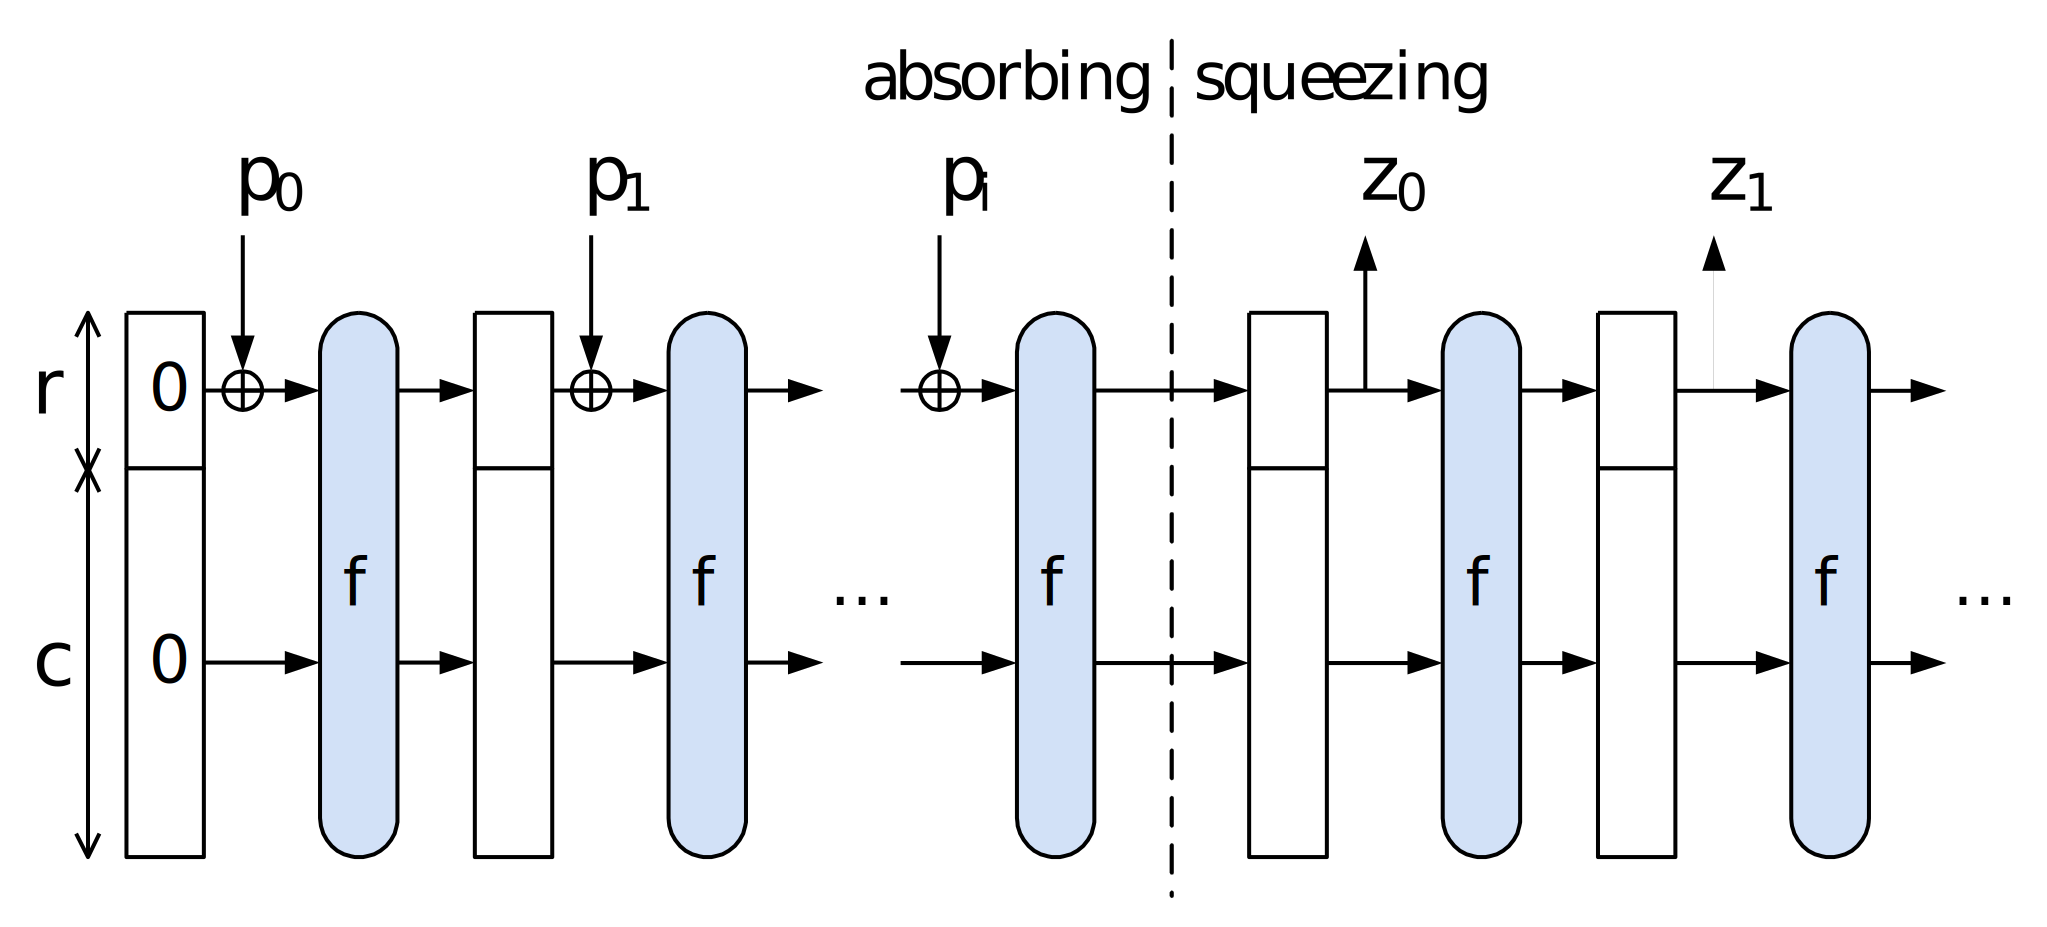
\includegraphics[width=110mm]{sponge-functions}
    \caption{Sponge function with rate $r$ and capacity $c$ absorbing a message $p$, outputting digest $z$.}\label{fig:sponge-functions}
\end{figure}

Keccak, in contrast to MD5 and SHA-1, is a sponge function, which means its internal structure is quite different from the traditional Merke-Damgård-based hash functions. Sponge functions have two phases, \emph{absorption} and \emph{squeezing}, and can be defined by their capacity $c$, the rate $r$, and their internal state size $s=c+r$, as illustrated in \autoref{fig:sponge-functions}. The higher the rate $r$, the faster messages will be absorbed and squeezed, as fewer steps through the permutation function $f$ are required. We can see that a construction like this does not enable re-construction of the internal state of the function from the bits squeezed, thus eliminating length extension attacks which make the \( h(key \| data ) \) pattern useless for Merkle-Damgård-based functions. The \(h(key \| data) \) pattern is how the Keccak designers recommend a MAC is constructed using Keccak \cite{sponge-functions}.

Keccak has an internal state size $s=1600$ bits, and can thus be fully specified by the rate. Keccak-$n$ indicates Keccak with $r=s-2n$, and an output size $n$. The strength of a sponge function is a function of its capacity, which will be 512 and 1024 bits for Keccak-256 and Keccak-512, respectively. We thus see that choosing parameters for Keccak is a speed-security trade-off, the higher the rate the better it'll perform, but at the cost of security.

While comparing these different solutions for generating MACs it's natural to also consider if there's any performance differences between them. A quick comparison of HMAC\footnote{The numbers were achieved by running the following command on the target platform: \texttt{python -m timeit -v -r 5 -n 1000 -s "msg = '10Bmessage'*10; import hmac, hashlib" "hmac.new('K'*16, msg, hashlib.sha1).digest()"}} vs. the different options for Keccak\footnote{Numbers achieved like this; substitute the 256 with 512 for the larger digest size: \texttt{python -m timeit -v -r 5 -n 1000 -s "msg = '10Bmessage'*10; import hashlib, sha3" "hashlib.sha3\_256('K'*16 + msg).digest()"}} and their performance on the target hardware is given in \autoref{tab:mac-perf-comparison}.

\begin{table}[ht!]
\caption{Performance comparison of different MAC implementations}\label{tab:mac-perf-comparison}
\centering
    \begin{tabular}{| c | c | c |}
    \hline
    \textbf{Scheme} & \textbf{Message size} & \textbf{Time} \\ \hline
    HMAC-MD5 & 100 B & 435$\mu$s \\ \hline
    HMAC-SHA1 & 100 B & 437$\mu$s \\ \hline
    Keccak-256 & 100 B & 87$\mu$s \\ \hline
    Keccak-512 & 100 B & 130$\mu$s \\ \hline
    HMAC-MD5 & 4 MB & 107ms \\ \hline
    HMAC-SHA1 & 4 MB & 169ms \\ \hline
    Keccak-256 & 4 MB & 1207ms \\ \hline
    Keccak-512 & 4 MB & 2208ms \\ \hline
    \end{tabular}
\end{table}

The rather abysmal performance of Keccak on the larger messages are not expected to be noticeable, since the underlying network is most likely going to be the bottleneck. When optimized the satellite can start sending bytes on the wire while performing the hash computation, and thus the hashing only needs to be faster than the underlying network. For the radio interface of an actual in-orbit satellite communicating over ham radio we're looking at bandwidths on the order of tens of Kbps, or likely less, which neither of the Keccak's will have any problem keeping up with. Another MAC could also be negotiated during the session establishment phase if an application in a different domain is restricted by Keccak performance. Note that one of the reasons for Keccak's poor performance on our Raspberry Pis is due to the \texttt{pysha3}-module not utilizing the optimized assembly code for ARM provided in the Keccak reference. Other implementations might have other performance characteristics; as always, benchmark if you're in doubt.

Keccak-$n$ as has a rate of \(1600-2n\), so the Keccak-256 tested had a rate of 1088 bits. Instead of MAC truncation like we're doing, this could be sped up by setting the internal Keccak sponge capacity to 128 bits and thus achieve a rate of 1472 bits, roughly 35\%  speedup. Note however that this is not supported in the \texttt{pysha3} module, as they only expose a traditional hashing interface to Keccak, and not to the underlying sponge function. Other implementations wanting to re-use the protocol, without the reference implementation provided here, are of course free to optimize this, at the cost of interoperability with other implementations.

For completeness, the current state of the art of breaking MAC-Keccak (Keccak as a MAC) is a cube attack against a reduced round (5 and 6 rounds) version of Keccak \cite{keccak_cube_attack}. The full version uses 24 rounds.


\section{Related Work}\label{sec:related_work}

This project builds mostly upon previous work done by other students working on the NUTS project, analyzing required security properties and suggesting protocols. The first of these was done by Visockas \cite{visockas} in 2011, who proposed a protocol using encryption for the uplink. Later Prasai \cite{prasai} rightfully showed in 2012 that confidentiality is unnecessary for access control, suggesting a protocol based on HMACs and sequence numbers. Later in 2012 the suggested protocol was tested on an ad-hoc radio link by Bezem and Fjellby \cite{bezem-fjellby}. In 2014 Münch picked up the task of implementing the suggested protocol \cite{marius-project}, and later trying to integrate it to the NUTS hardware \cite{marius}. However, this implementation moved away from the complexities of the sequence numbers and the problematic synchronization routines suggested previously, in favor of a system based on broadcast timestamps. In contrast to the previous work though, this work does not have a way to authenticate the downlink, and was thus not found to satisfy the desired properties of the protocol.

The protocol suggested here bears many similarities to \gls{tls}, and in particular it's datagram-based variant \gls{dtls}. TLS is the most widely deployed protocol on the Internet for secure communication, and has had years of scrutiny of both the protocol and several implementations. DTLS is very similar to it's stream-oriented sibling, sharing the same message construction and many of the same cipher suites, apart from stream ciphers like RC4. Environments with constrained resources -- like satellites and their radio links -- is exactly the motivation for standards like \gls{psk} over DTLS \cite{rfc4279}. Combining this with NULL encryption cipher suites like TLS\_ECDHE\_PSK\_WITH\_NULL\_SHA256 \cite{rfc5489} would thus yield a protocol very similar to \gls{nap}. Hence, it's worth pointing out how this would differ from our protocol.

The (D)TLS record layer adds a three byte header to it's message; one byte packet type and two bytes for the length. There's also a tailing MAC with the length being equal to the digest of the MAC algorithm, thus yielding a 20 byte MAC for SHA-1 or 32 bytes for SHA-256. The protocol suggested in this paper only has two bytes of header, and a customizable 4--32 bytes of MAC, depending on the required strength in a given deployment. Our protocol thus requires less bandwidth than its (D)TLS equivalent. Granted, using (D)TLS extensions it's possible to negotiate a truncated MAC \cite{tls-extensions} reducing the MAC overhead of (D)TLS slightly, but the MAC can only be truncated to a fixed size of 10 bytes.

It's also worth noting that DTLS implementations are not as widely available as the TLS equivalent. Only recently have popular libraries started to gain support for DTLS, but several of the most common libraries such as OpenSSL and PolarSSL does not support it yet as of yet (December 2014). Among implementations which support DTLS1.2 it gets patchy when you look for specific cipher suites supported. CyaSSL for example supports DTLS1.2, but not (EC)DHE-PSK. This is a significant barrier for utilizing DTLS1.2 for our use case, as trying to extend existing TLS libraries without prior experience from development on the libraries is non-trivial.

It must also be said that writing things from scratch and not relying on existing work seems to be the spirit in which work is done on the NUTS platform, a practice that can be defended by the project's learning goals. It's also beneficial to start fresh and not carry around on the luggage (D)TLS has carried around since its early SSL days, like the MAC-then-encrypt structure that's been the source of heaps of attacks towards TLS lately (\cite[Lucky Thirteen]{lucky-thirteen}, \cite[BEAST]{beast}, \cite[CRIME/BREACH]{breach}, \cite[POODLE]{poodle}). Note however that none of these attacks apply to an authentication-only scheme, which might be due the lesser number of deployments with such schemes, and thus limited research interest in the topic.

Future applications might want to investigate whether DTLS has reached a mature enough state to be useful and implemented in popular libraries.
